\documentclass[a4paper]{article}
\usepackage[utf8]{inputenc}
\usepackage[spanish]{babel}

\usepackage{graphicx,psfrag}
\usepackage{amsfonts,amssymb,amsthm,amsmath}
\usepackage{fullpage}

\usepackage[hidelinks,breaklinks]{hyperref}
\hypersetup{
  citecolor=blue,
  citebordercolor={1 1 1},
  linkbordercolor={0 1 0},
  pdfborder={0 0 0.5 [3 3]},
  colorlinks=true
}

\title{Poncho para Arduino/Galileo -- ponchitoCIII}
\author{Gonzalo F. Perez Paina (CIII-UTN-FRC)}
\date{\today}

\begin{document}
\maketitle
%\tableofcontents

\section{Introducción}
Las mayoría de las placas de desarrollos disponibles en el mercado cuentan con una variedad de placas adicionales que permiten expandir las funcionalidades básicas.
Estas placas reciben diferentes nombre tales como: placas de expansión o daughter board, shield --particularmente en el proyecto Arduino~\cite{Arduino}--, o poncho --en el proyecto EduCIAA~\cite{EduCIAA}--.
La placa que se describe aquí sirve de expansión para Arduino o Intel Galileo~\cite{Galileo}. 

\section{Objetivo}
%El objetivo principal es realizar una donación de un total de 20 unidades de la placa ponchitoCIII al Laboratorio de Técnicas Digitales del Departamento de Ingeniería Electrónica de la UTN-FRC.

El objetivo de la placa es contar con el hardware necesario para realizar las primeras prácticas en programación sobre sistemas embebidos. 
Se puede utilizar para el desarrollo de software con los esquemas de \texttt{sketch} de Arduino (con placas Arduino o Intel Galileo), programación en lenguaje C de los microcontroladores AVR de las placas Arduino (sin el IDE Arduino), como así también para la programación de Linux embebido sobre la Intel Galileo.

\section{Descripción}
El ponchitoCIII cuenta con componentes adicionales similares a los disponibles en la EduCIAA, tales como: LEDS con los colores de semáforos (rojo, amarillo y verde), pulsadores, y potenciómetro como entrada al conversor analógico a digital.

La figura~\ref{fig:ponchito} muestra el ponchitoCIII con los diferentes componentes.
También se indican los pines de alimentación (GND y Vin) que sirve como referencia para insertar esta placa en la placa madre (Arduino o Intel Galileo).
\begin{figure}[hbt]
  \centering
  \psfrag{a}[rB][rB]{LED rojo}
  \psfrag{b}[lB][lB]{LED amarillo}
  \psfrag{c}[lB][lB]{LED verde}
  \psfrag{d}[rB][rB]{Pulsador izquierdo}
  \psfrag{e}[rB][rB]{Pulsador central}
  \psfrag{f}[lB][lB]{Pulsador derecho}
  \psfrag{g}[lB][lB]{Potenciómetro}
  \psfrag{h}[c][c]{5V}
  \psfrag{i}[][]{GND}
  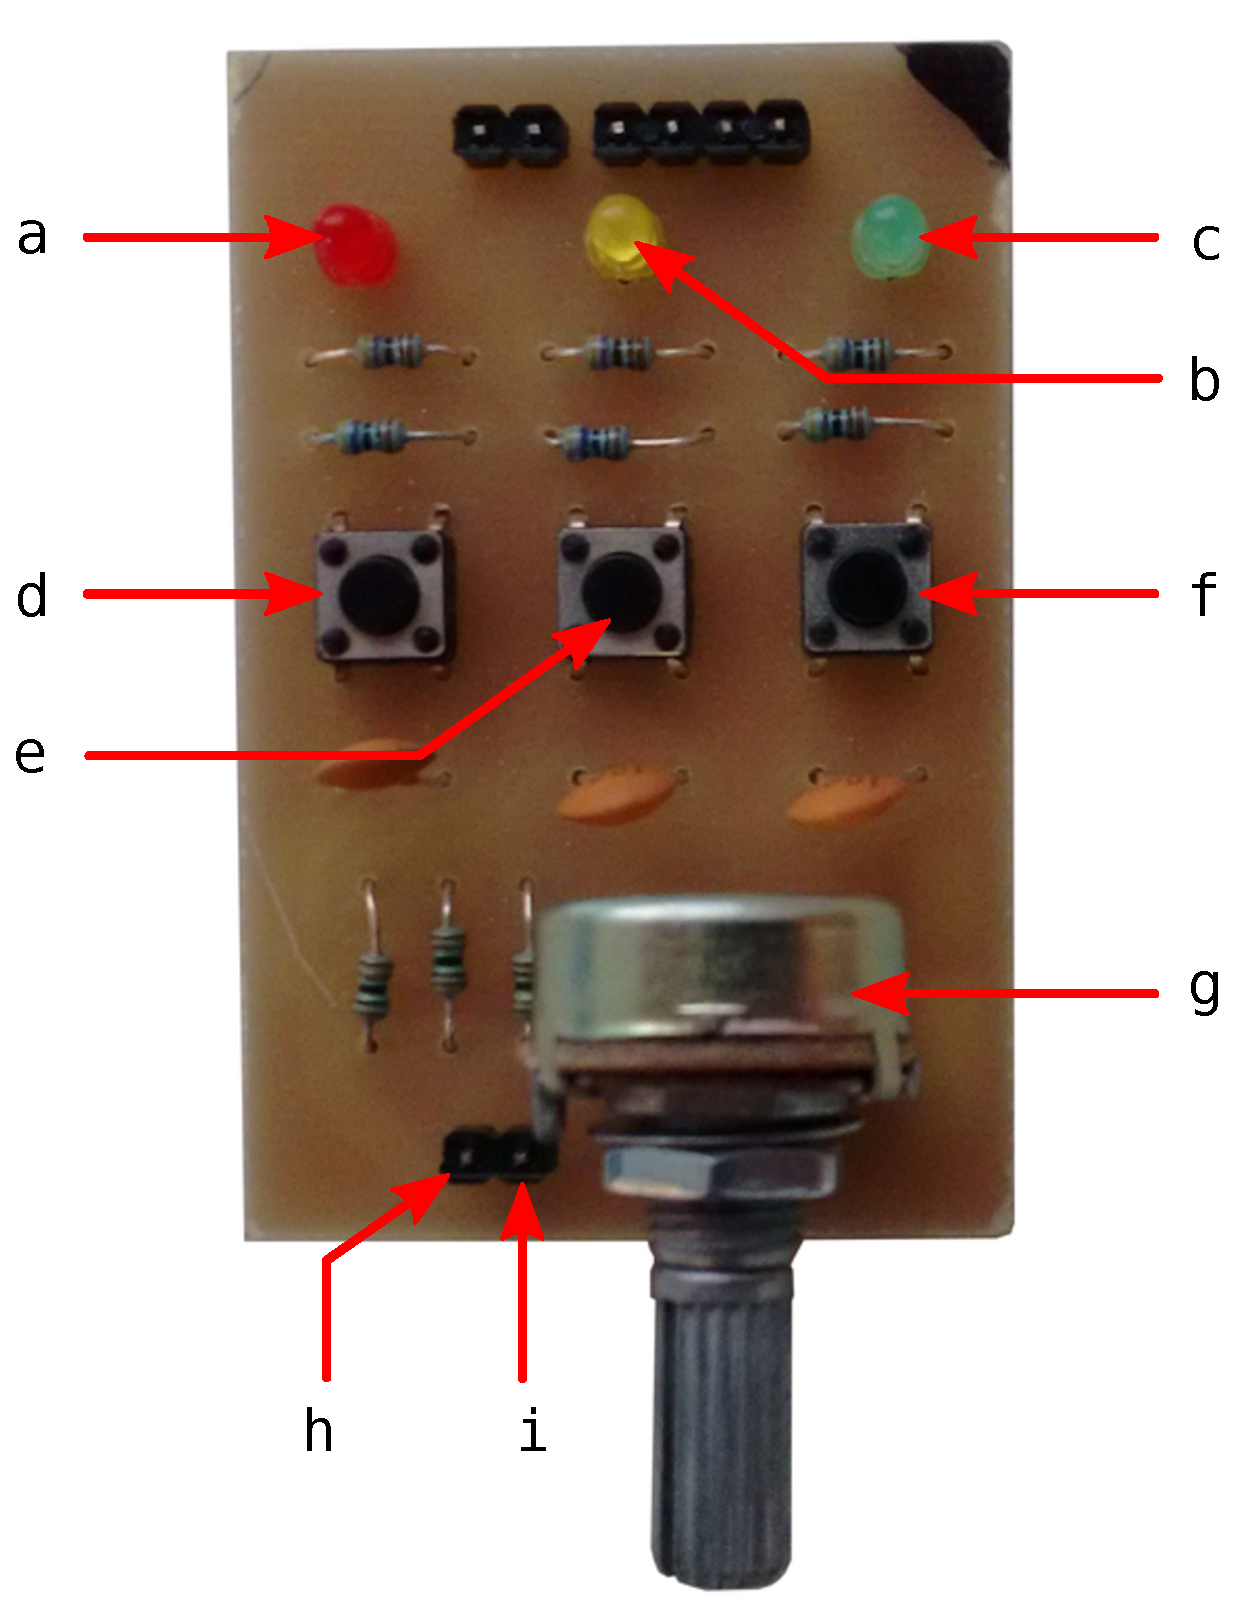
\includegraphics[width=0.30\textwidth]{ponchito.eps}
  \caption{Detalle del ponchitoCIII.}
  \label{fig:ponchito}
\end{figure}

\bigskip
A continuación se indican las conexiones de los diferentes componentes:
\begin{itemize}
  \item  LED verde: \texttt{Pin 5 (PWM$\sim$)}
  \item  LED amarillo: \texttt{Pin 6 (PWM$\sim$)}
  \item  LED rojo: \texttt{Pin 9 (PWM$\sim$)}
  \item  Pulsador izquierdo: \texttt{Pin 8}
  \item  Pulsador central \texttt{Pin 7}
  \item  Pulsador derecho: \texttt{Pin 4}
  \item  Entrada analógica/potenciómetro: \texttt{Pin A0}
\end{itemize}

Este documento como también algunos sketch Arduino de ejemplos para evaluar la placa se encuentra disponibles en \href{https://github.com/ciiiutnfrc/ponchitoCIII}{https://github.com/ciiiutnfrc/ponchitoCIII}.

\section*{Agradecimientos}
El diseño del circuito y del PCB, la fabricación de los PCB, el montaje y evaluación de las placas se llevó a cabo en el Laboratorio de Electrónica del Centro de Investigación en Informática para la Ingeniería (CIII) de la Facultad Regional Córdoba de la Universidad Tecnológica Nacional (UTN-FRC).
Gracias a Axel Schneider quien estuvo a cargo de la fabricación de los PCB, a Ariel Zsilavecz y Julio Sanchez, todos alumnos de la carrera de Ingeniería Electrónica en la UTN-FRC, quienes montaron y evaluaron el correcto funcionamiento de las placas, y a Facundo Navarro quien actualizó el diseño del PCB a la versión de KiCAD 5.0.

\begin{thebibliography}{9}
  \bibitem{Arduino} Arduino. \href{http://www.arduino.cc/}{http://www.arduino.cc/}
  \bibitem{EduCIAA} La CIAA en la educación. \href{http://www.proyecto-ciaa.com.ar/devwiki/doku.php?id=educacion}{http://www.proyecto-ciaa.com.ar/devwiki/doku.php?id=educacion}
  \bibitem{Galileo} Intel Galileo. \href{https://www.arduino.cc/en/ArduinoCertified/IntelGalileo}{https://www.arduino.cc/en/ArduinoCertified/IntelGalileo}
\end{thebibliography}

\vfill
\begin{flushright}
  \LaTeX~/~Creado en noviembre de 2017
\end{flushright}

\end{document}

